\documentclass[12pt, fleqn]{article}

\usepackage[left=0.75in, right=0.75in, bottom=0.75in, top=1.0in]{geometry}
\usepackage{amsmath}
\usepackage{amssymb}
\usepackage{amsthm}
\usepackage{mathtools}
\usepackage{hyperref}
\usepackage{ulem}
\usepackage{enumitem}
\usepackage{floatrow}
\usepackage{graphicx}
\usepackage[export]{adjustbox}
\usepackage{sectsty}
\renewcommand{\thesubsubsection}{(\alph{subsubsection})}

\usepackage[dvipsnames]{xcolor}
\usepackage[perpage]{footmisc}

\usepackage{fancyhdr}
\pagestyle{fancy}
\fancyhf{}
\lhead{190100044}
\rhead{Assignment 1}
\renewcommand{\footrulewidth}{1.0pt}
\cfoot{Page \thepage}

\setlength{\parindent}{0em}

\title{Assignment 1}
\author{Devansh Jain, 190100044}
\date{29 Aug 2021}

\newcommand{\twoxone}[2]{
    \begin{pmatrix}
        #1 \\
        #2
    \end{pmatrix}
}

\begin{document}

% \pagenumbering{gobble}
\maketitle
\tableofcontents
\thispagestyle{empty}
\setcounter{page}{0}

\newpage
\section{Ordinary Least Squares (OLS) Regression in one variable}
Notation: \\
$\mathbf{X}$ is $N \times 1$ vector, \\
$\mathbf{Y}$ is $N \times 1$ vector, \\
$\mathbf{1_N}$ is $N \times 1$ vector (all 1s), \\
$x_i$ is scalar (i$^\text{th}$ observed sample), \\
$y_i$ is scalar (i$^\text{th}$ observed output), \\
$w$ is scalar, \\
$b$ is scalar.

\subsection{CS337: Theory}
\begin{equation*}
  \begin{aligned}
    mse(w,b)                             & = \frac{1}{N} \sum_{i=1}^N ((w x_i + b) - y_i)^2                                                                                                    \\
    \frac{\partial mse(w,b)}{\partial w} & = \frac{1}{N} \sum_{i=1}^N 2 \ ((w x_i + b) - y_i) \ x_i                                                                                            \\
                                         & = \frac{2}{N} \sum_{i=1}^N (w x_i + b - y_i) \ x_i                                                                                                  \\
                                         & = \frac{2}{N} \ \text{dot}(w \mathbf{X} + b \mathbf{1_N} - \mathbf{Y}), \mathbf{X})                                                                 \\
    \frac{\partial mse(w,b)}{\partial b} & = \frac{1}{N} \sum_{i=1}^N 2 \ ((w x_i + b) - y_i)                                                                                                  \\
                                         & = \frac{2}{N} \sum_{i=1}^N (w x_i + b - y_i)                                                                                                        \\
                                         & = \frac{2}{N} \ \text{sum}(w \mathbf{X} + b \mathbf{1_N} - \mathbf{Y})                                                                              \\
    \nabla mse(w,b)                      & = \twoxone{\frac{\partial mse (w,b)}{\partial w}}{\frac{\partial mse (w,b)}{\partial b}}                                                            \\
                                         & = \frac{2}{N} \twoxone{\text{dot}(w \mathbf{X} + b \mathbf{1_N} - \mathbf{Y}), \mathbf{X})}{\text{sum}(w \mathbf{X} + b \mathbf{1_N} - \mathbf{Y})}
  \end{aligned}
\end{equation*}

\subsection{CS335: Lab}
\subsubsection{}
Code for the function \verb!split_data()! updated in notebook.

\subsubsection{}
Code for the function \verb!mse_single_var()! updated in notebook.

\subsubsection{}
Code for the functions \verb!singlevar_grad()! and \verb!singlevar_closedform()! updated in notebook.
\begin{figure}[H]
  \centering
  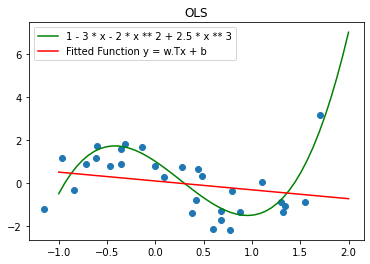
\includegraphics[scale=0.7]{singlevar_grad.png}
  \caption{Single Variable Regression - Gradient Descent (\texttt{epochs}=1000, \texttt{lr}=1e-2)}
\end{figure}
\begin{figure}[H]
  \centering
  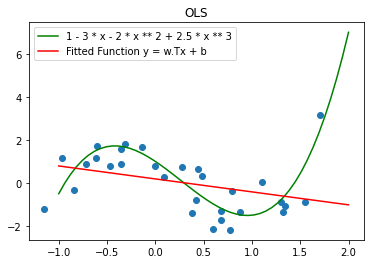
\includegraphics[scale=0.7]{singlevar_closedform.png}
  \caption{Single Variable Regression - Closed Form}
\end{figure}

\subsubsection{}
As mentioned in description of the question (point 5), the error function (mse) is convex and has just one minimum. \\
By using the closed form, we get the point corresponding to minimum mse error. As we compute the parameters based on training data, the training loss is minimum at this point. \\
Therefore, training loss for solution of \verb!singlevar_grad()! can never be strictly less than that of the solution obtained by \verb!singlevar_closedform()!.

\end{document}
